\chapter{How To Write A Visualization Survey Paper: A Starting Point}
\label{chap:howTo}
\bibentry{mcnabb2019how} \cite{mcnabb2019how} \\
%% Restart the numbering to make sure that this is definitely page #1!
\pagenumbering{arabic}

\begin{abstract}
This paper attempts to explain the mechanics of writing a survey paper in data visualization or visual analytics. It serves as a useful starting point for those who have never written a survey paper or have very little experience. A literature review or survey paper is often considered the starting point of a PhD candidate's scientific degree. However, there are no dedicated papers that focus on guidelines for the planning or writing a survey paper or literature review in visualization or visual analytics. We provide guidelines and our recommendations for a foundational structure on which to build a survey paper, whilst also considering intermediate goals, and offer helpful advice to improve the  survey process and literature analysis. The result is a useful starting point for those wishing to write a survey paper or state-of-the-art (STAR) review in visualization or visual analytics. The guidelines and recommendations we make can also be generalized to other areas of computing and science.\\

An abstract is a required feature of a survey paper and should identity the topic of the literature review. A good abstract addresses why the given topic is interesting and why it is helpful. A good abstract features the following elements:  (1) topic introduction, (2) the motivation, (3) the goal of the review, and the benefits the review provides to the reader. A good literature survey offers a helpful classification of the literature, mature areas of research, and open, unsolved  problems in visualization or visual analytics.
\end{abstract}  \newpage
%-------------------------------------------------------------------------
\section{Introduction and Motivation} \label{sec:introduction}
A survey paper is an incredibly useful tool for both newcomers and experts of a given field. Twenty years ago, Jim Blinn stated \emph{"There's lots of other journals and it takes more and more effort to make sure that you know what's happening."} \cite{blinn1998ten} One of a survey paper's primary goals is to assist the reader in the hunt for  previously published research papers on a given topic.We discuss a general approach to planning and writing a typical survey paper section-by-section, and provide  more details and guidelines as to appropriate content in each section. 

The target audience of this paper is a PhD student in their first year and their supervisor. This paper presents and follows a versatile template which the reader can follow to accelerate and facilitate the creation of a survey paper. In addition, we discuss important considerations in the preparation phase of a survey paper. For this, we use the symbol (\cons) to designate aspects that are examined as part of the preparation, but are not necessarily  discussed in the actual the text itself. The guidelines and recommendations are based on our experience of reading and writing survey papers in visualization \cite{post2003state, laramee2004state, laramee2007topology,  peng2009higher, mcloughlin2010over, edmunds2012surface, lipsa2012visualization, borgo2013glyph, chung2014glyph, tong2018storytelling, firat2018towards, roberts2018visualising, rees2019survey} as well as meta-surveys, or surveys of surveys (SoS) \cite{mcnabb2017sos, alharbi2017molecular, alharbi2018sos}.


 A well written introduction motivates the topic, including applications of the topic, why the research direction is important, and what the contributions of the survey or state-of-the-art (STAR) report are. Here we use the term "STAR" to refer to literature reviews with a special focus on recent literature, e.g, within the last 10 years. Survey papers are more comprehensive and may include literature from all years.
%\textbf{Paper Titles:} A paper title is an important decision. The title must easily present the paper's topic as well as allow quick communication between researchers. We use \emph{`Survey of Surveys (SoS) - Mapping The Landscape of Survey Papers in Information Visualization'} as one standard example \cite{mcnabb2017sos}. The main title gives a frank understanding of the topic area, coming with an additional acronym for easy conversation or reference, and follows up with a subtitle to give further context.  If the topic is clear, a different approach can use \emph{`Document Visualization: An Overview of Current Research'} as an example\cite{gan2014document}. Where the main title is the core field, followed by the type of survey produced.

The introduction and motivation describe some of the big research challenges that are faced by the topic covered by the survey. Some generic aspects that can be considered common challenges are: the rapidly increasing size and complexity of the data, heterogeneous data sources, uncertainty, challenges associated with equipment such as cost or speed, cognition and perception, understanding or representation of observations, the limitations of existing software, and hardware or software performance limitations.

\subsection{Contributions}
The contributions are clearly presented in either the introduction (and motivation) section or a subsection. A reader can recognize the importance and novelty of any paper by the end of the introduction and the insight and benefits that can be gained from reading it. We recommend authors strive for approximately three contributions. These contributions are described in conjunction with the rest of the first section, to make it clear how the survey paper fits into the visualization field's landscape. Examples of a typical contribution include: 
\begin{itemize}
\item A novel classification of the literature (how your classification differs from previous surveys, or whether the survey is the first of it's kind in the field).
\item A compilation of future challenges or trends in the domain.
\item The identification of both mature and less explored research directions in the field.
\end{itemize}


A good review paper considers key questions in the field. What has been published so far? Are there any controversies, debates or contradictions that should be brought to light? Which methodologies have researchers used, and which appear to be best? Who are the leading experts in the field? And how the topic fits into the landscape of visualization. By analyzing questions like these, your survey presents some clear contributions to discuss.

The contributions of this paper include: 

\begin{itemize}[labelindent=0em, labelsep=0.2cm, leftmargin=*]
\item[\textbf{1.}] The first guidelines (to our knowledge) on how to write a survey paper in data visualization or visual analytics.
\item[\textbf{2.}] Guidelines on the process of preparing a literature survey.
\item[\textbf{3.}] A structured survey paper template that can be followed, with in-depth guidelines describing the content of each section.
\end{itemize}

\textbf{Temporal Planning \cons :} We believe a high quality, full survey paper can take approximately a full year (part-time) to incrementally prepare and write including the literature search. A significant portion of this time concentrates on gathering the related literature on a given literature review topic. Due to the length of full survey papers (20-30 pages), it is time-consuming and difficult to undertake multiple internal full paper reviews and revisions, therefore it is helpful to distribute the preparation, discussion and intermediate feedback sessions periodically over the preparation time frame, to reduce the drafting and corrections process in the final stages. A tested strategy can separate the individual paper browsing and summarization process from the main survey paper organization \cite{laramee2010write}. Individual research paper summaries can be written on a weekly basis for the first six months, yielding roughly 24 summarized topic papers before any final decisions have been made on the organization, or literature classification. This provides a good basis for potential paper classifications to develop.

%\textbf{Latex:} \LaTeX~is a tool for writing high-quality papers at a professional level. The majority of conferences at this point provide a standard latex template to work with, allowing your paper to hit the standard at which the conference desires. If you, or the main author are not confidant with \LaTeX, then the strategy presented above may allow for steady progress before the bulk of the survey is attempted.
\subsection{Challenges of Writing a Survey} \label{sec:challenges}
We identify seven main challenges associated with writing a survey paper. 
\begin{itemize}[labelindent=0em, labelsep=0.2cm, leftmargin=*]
\item[\textbf{1.}] Managing the amount of previously published literature (discussed throughout this paper)
\item[\textbf{2.}] Identifying a starting point (the purpose of this paper)
\item[\textbf{3.}] Deciding on a topic (see Scope, Section \ref{sec:scope})
\item[\textbf{4.}] Performing a search (see Search Methodology, Section \ref{sec:search})
\item[\textbf{5.}] Interpreting individual research papers (see Section \ref{sec:summary})
\item[\textbf{6.}] Deriving a classification of literature on the given topic (see Section \ref{sec:classification})
\item[\textbf{7.}] Determining related unsolved problems and future challenges (see Section \ref{sec:fut})
\end{itemize}

In the following sections, we address some of these central challenges.

\subsection{Literature Search Methodology \cons} \label{sec:search}
It is important to clearly describe how you search for the papers cited in the survey. When a reader browses the literature review, it is likely that you have found research papers that they may not have seen. A new PhD student usually has not yet discovered all of the relevant conferences and journals to search. The literature search methodology provides the names of digital libraries, search engines, search terms, and literature sources used to find literature in your survey paper. 
If we are looking for research papers on the topic of treemaps, we can use the Google Scholar search engine for example \cite{scholar} to search the term "treemap". This gives us (at the time of writing) over 16,000 related search results. By doing the same using the IEEE Xplore Digital Library \cite{ieeexplore}, we get 115 items, and using vispubdata \cite{isenberg2017VPD}, we get 58 items. For visualization purposes, the three previously-mentioned search engines are a great tool, combined with the use of Google Scholar's "Cited by..." option to find related work, you should be able to gather a fairly complete set of papers. A complete list of sources to search is provided in Table \ref{table:searchTable}.

\begin{table}[t]
\ra{1.2}
\footnotesize
\centering
\rowcolors{1}{white}{black!3}
\begin{tabularx}{0.6\textwidth}{|X|}
\hline \rowcolor{black!30}
Literature Sources \\ \hline
%\rowcolor{black!30}  &  Papers \\ 
Google Scholar  \cite{scholar}\\
IEEE Xplore Digital Library \cite{ieeexplore}\\
ACM Digital Library \\
Vispubdata \cite{isenberg2017VPD}\\
The Annual EuroVis Conference   \\
IEEE TVCG Journal  \\
IEEE Pacific Visualization Symposium  \\
IEEE VAST Conference  \\
The Annual Eurographics Conference  \\
The Eurographics Digital Library \\
Journal of Visual Languages \& Computing  \\
Information Visualization Journal  \\
Computer Graphics Forum  \\
Computer \& Graphics \\
ACM Computing Surveys  \\ 
\hline
\end{tabularx}
\caption{A shortlist of literature sources.} \label{table:searchTable}
\end{table} 

The other search consideration is a manual search. When you have found one matching paper, it is likely that you will find a number of related research papers in the related work of the given match. This can be especially useful if there are related survey papers. If you find the majority of papers this way, providing a breakdown of conferences and journals may be a beneficial method of presenting your literature search. The goal is to provide enough information to make your literature search thorough and reproducible. 

\subsection{Literature Classification Overview}  \label{sec:overview}
Organizing the research papers in your survey is a central topic in any literature reviews. Classification dimensions can be derived for the task.
Each of your classification dimensions is presented in this section. One dimension of a literature classification is often a list of (subjects or) topics. Describe each topic in the classification, how each research paper is classified, and possibly some exceptions where research fits into multiple subject categories. A high-quality literature classification is often composed of more than one dimension, e.g. subject category and data dimensionality. By talking about dimensions separately, you allow the reader to understand what is presented in the classification before discussing the individual topics and papers. Images or tables are a good way of conveying an overview.

Refer to McNabb and Laramee's Survey of Surveys for an example \cite{mcnabb2017sos}. One axis consists of an adapted Information Visualization pipeline. A second dimension is a set of topic clusters. A section is presented to to discuss how their pipeline differs from Card et al.'s original \cite{card1999readings}, and why modifications have been made. The topic clusters are discussed in a separate section. How the subjects were gathered and selected is explained. Both sections provide a visual representation to aid in the understanding of each main axis.

It is important to clearly explain each axis of your proposed literature classification as this is one of the most important aspects of a survey paper which can clearly impact whether a survey paper makes it through the review process. Please review Section \ref{sec:classification} for a detailed guide to developing a classification.
 
\subsection{Survey Scope \cons} \label{sec:scope}
Defining the scope of a survey -- subject categories or the topics it covers (and does not cover) can be a very challenging aspect of writing any literature review. The scope defines the topic boundary of literature that is included and excluded from the survey. If the scope is too broad, then the survey includes too many research papers to manage. If the scope is too narrow, then not enough literature may be included for a good classification from which deductions may be drawn. Therefore, it is important to accurately designate what does and does not meet the scope of your paper. The scope is flexible as long as you clarify the scope boundaries clearly. For example, if you paper reviews a specific topic of interest (i.e. a technique or application), then it makes sense to explicitly state that this is the case.

% On the other hand, if you find fringe topics, it may be best to leave these out. If a paper opens a door to a new set of papers, it may be best to leave those out.
Aim to create a scope that encompasses roughly 40-50 research papers. If you cannot see any avenues of narrowing your scope, year of publication is always an option and can be used as a soft-cap, for example, Alsallakh et al.\ with their state-of-the-art in sets and set-typed data \cite{alsallakh2014visualising}. Limiting your survey to the most recent 10 years also turns it into a STAR. Doing this can be a way of reducing the focus research papers while still including older papers for other types of analysis if necessary. Provide examples when pointing out what is and isn't in scope. Lipsa et al.\ provide an informative example of a scope \cite{lipsa2012visualization}. The survey clears presents papers that do or do not meet the scope criteria, with given examples of papers.

A very common problem is defining a scope that is too broad. We recommend a scope that includes approximately 50 research papers per PhD student and supervisor pair on the author list. You can use Google Scholar and the other search engines described in Section \ref{sec:search} to make early assessments of scope. For example, if you enter "Isosurface" into a search engine for research papers, you will get a broad scope including over 100 research papers. The scope could be narrowed by focusing on isosurfaces for time-dependent data.

\textbf{Survey Type \cons :} It is important to consider the type of survey that you would like to present within your scope. A \textit{`Literature Review'} refers to a more comprehensive list of papers on a given research direction whilst a \textit{`State-of-the-Art'} (STAR) report refers to the more recent research or techniques. Some examples of this include  Beck et al.\ with their state-of-the-art in visualizing dynamic graphs \cite{beck2014state} and Laramee et al.\ with the state-of-the-art in flow visualization \cite{laramee2004state}. On top of this surveys can focus on task taxonomies rather than the field itself. Examples of this include Kerracher et al.\ and their task taxonomy for temporal graph visualization \cite{kerracher2015task}, or Schulz et al.\ with their design space of visualization tasks \cite{schulz2013design}. These are important considerations to discuss with any potential co-author.

\begin{figure}
\centering
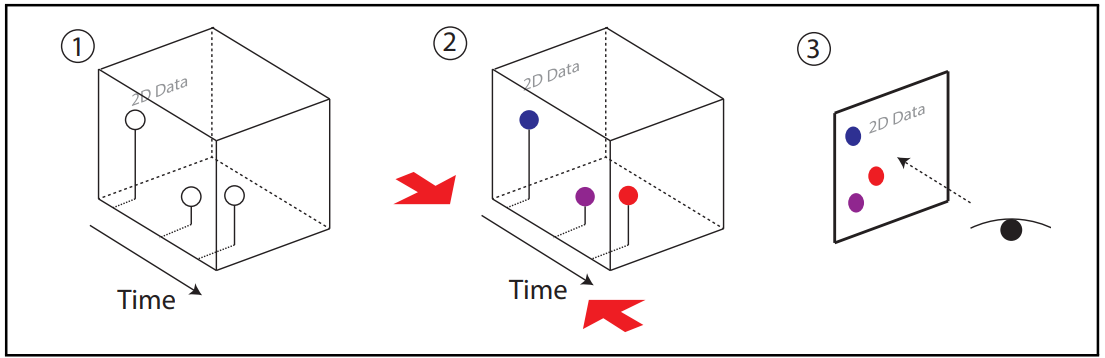
\includegraphics[width=1\linewidth]{pictures/sto.png}
\caption{The colored time flattening operation for space-time cubes. An example depicting a technique using visual rerpresentation. Image courtesy of Bach et al.\ \cite{bach2014review}} \label{fig:sto}
\end{figure}

\subsection{Survey Paper Organization}
The organization of the survey refers to the order in which research papers and subject topics are presented in the main body of the literature review. Organization of a survey can be trivial when the classification has been developed. Research topics and papers can be discussed in linear order based on the primary dimension in your classification, where the secondary dimension will represent the sub-sections of your survey. In each section, a sub-organization can be applied either based on another classification or publication year. Tong et al.\  present their classification dimensions and follow chronological order when presenting their summarized research papers in each sub-section \cite{tong2018storytelling}. 

\section{Related Work} \label{sec:related}
There are a number of other related educational papers readers may find very useful.
Sastry and Sastry develop a tool named a summary-comparison matrix (SCM) to aid in the organization and extraction of information in research papers \cite{sastry2013summary}. Our paper differs to this by contextualizing the entire survey writing process.
Laramee presents a starting point on how to write an individual visualization research paper \cite{laramee2010write}. The paper covers each aspect of the individual paper including the introduction, method, implementation, and performance. The paper also covers important considerations such as planning, procedure diagrams, figures and images, and supplementary material. This paper is considered sibling reading and is encouraged for discussions on paper writing, titles, latex, and collaboration. Laramee also presents guidelines on how to read and summarize a visualization research paper \cite{laramee2011read}. We extend this in Section \ref{sec:summary} to guide uses in extracting the essentials of a survey paper. Daniel Patel provide an educational paper focused on the requirements of an article-based PhD in visualization \cite{patel2011phd}. Munzner provides an overview of pitfalls authors may fall into, leading to rejection during the reviewing process \cite{munzner2008process}.


\subsection{Background}
Depending on your chosen topic, it may be appropriate to include about a background section. A background section reviews the history of a topic such as how a technique originally emerged and it's evolution, or how its use has changed.  Nusrat and Kobourov give an excellent example by looking at the evolution of cartograms in the 19th and 20th century \cite{nusrat2016state}. Borgo et al present the history of glyphs and their applications \cite{borgo2013glyph}.

%\textbf{Collaboration \cons :} Collaboration is a good process for enabling a wider literature search and increasing the quality of the paper.
\section{Presenting the Main Literature Survey}\label{sec:presenting}
Section \ref{sec:presenting} discusses individual research papers, developing a literature classification, and different types of paper classification.
\subsection{Summarizing An Individual Research Paper} \label{sec:summary}
This sub-section is adapted from the paper by Laramee and focuses on extracting essential information from a single visualization paper \cite{laramee2011read}. This is a helpful exercise during both the preparation and writing phases of a literature review. It also facilitates the development of a literature classification (Section \ref{sec:classification}). We extend this to provide guidance when summarizing an individual survey paper based on the experience gathered writing the SoS \cite{mcnabb2017sos}. This is helpful for describing survey papers  that may be included in the related work section (Section \ref{sec:related}). When summarizing an individual research paper, the core elements to extract are: the concept, related work, data characteristics, visualization techniques, and application domain. 

The focus elements of a survey paper vary in what may be considered the important essentials or aspects. For example, it is unlikely that a survey has a regular set of data characteristics. For a survey we focus on: the concept, the scope, the classification, classification dimensions, and unsolved problems or future work. Here is a sample survey summary of space-time cube operations by Bach et al.\ \cite{bach2014review} 

%\begin{tcolorbox}[title=\textit{A Review of Temporal Data Visualizations Based on Space-Time Cube Operations} by Bach et al. \cite{bach2014review}]
\begin{footnotesize}
Title: \textit{A Review of Temporal Data Visualizations Based on Space-Time Cube Operations} by Bach et al. \cite{bach2014review}
\begin{enumerate}
\item \textit{The Concept:}
Bach et al.\ survey a variety of temporal data visualization techniques and discuss how their operations represented by space-time cubes are used in the context of a volume visualization from the 2D+time model. \cite{bach2014review}
\item \textit{The Scope:}
The paper discusses common space-time cube operations including time-cutting, time flattening, time juxtaposition, space cutting, space flattening, sampling, and 3D rendering. Bach et al.\ then present the taxonomy of space-time cube operations they designed before providing the reader a selection of multi-operation systems.

\item \textit{Classification:}
The taxonomy (<Figure 24 of original paper>) presents a classification of elementary space-time cube operations such as drilling, cutting and chopping. These are broken down into sub-categories with schematic illustrations in order to enable the user to easily understand what effect the operation has. For example, the flattening section is broken down into planar flattening and non-planar flattening. Planar flattening is sub-divided into orthogonal flattening and oblique flattening.

\item \textit{Figure: <Figure 24 of original paper> }
%\begin{figure}[p] 
%\begin{center}
%\includegraphics[width=1\textwidth]{images/bach2014reviewFull}
%\caption{Taxonomy of Space-Time cube operations created by Bach et al.\ \cite{bach2014review} Each operation gives a representation of how the operation may work. Bold font indicates complete operations. Gray shading indicates non-leaf nodes. Image courtesy of Bach et al.\ \cite{bach2014review}} \label{fig: bach2014review}
%\end{center}
%\end{figure}

\item \textit{Classification Dimensions:}
\begin{itemize}
\item[X-Axis:] Operations, Time, Space
\item[Y-Axis:] Extraction: [Point Extraction, Planar Drilling, Planar Cutting, Non-Planar Cutting, Planar Chopping, Non-Planar Chopping],\\
Geometry Transformation: [Rigid Transformation, Scaling, Bending, Unfolding],\\ 
Content Transformation: [Recoloring, Labeling, Re-positioning, Shading, Filtering, Aggregation],\\
Flattening, Filling.
\item \textbf{Supplementary URL:} \url{http://spacetimecubevis.com/}
\item \textbf{Papers:} There are 91 Papers cited in the survey (1970-2013)\\
\end{itemize}

\item \textit{Unsolved Problems/Future Research:}
There are many open research areas discussed. Some of these include interaction techniques such as focus+context applied to different operations, research into operations for extended data dimensions, and understanding which operation is most appropriate for a given task.

\end{enumerate}
\end{footnotesize}
%\end{tcolorbox}

You can see the initial summary follows a template. This is useful for treating the survey papers systematically including collecting meta-data in a consistent and helpful manner. When the papers start to be placed into the survey, the template format can be adjusted into  more naturally written text.

\begin{figure}
\centering
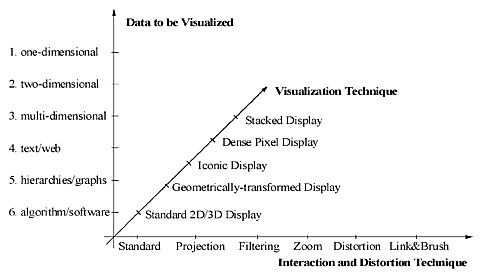
\includegraphics[width=1\linewidth]{pictures/techniquetaxonomy.png}
\caption{Keim's 
Classification of information visualization techniques. Courtesy of Keim \cite{keim2002information}. } \label{fig:keim}
\end{figure} 


\subsection{Developing a Literature Classification (How To) \cons } \label{sec:classification}
%\highlight{Refer to Video}
Deriving a literature classification is one major challenge of writing a survey. A classification categorizes each research paper such that similar papers fall into the same group. Deriving groups, categories, and dimensions for your classification requires careful thought.

One property of a good classification is that it is easy to properly place research papers into categories. If you have great difficulty placing individual research papers into the categories identified in your classification, this may be a sign that it requires adjustment.

\subsection{Identifying Classification Dimensions \cons } \label{sec:identify}
There has been a lot of work invested in generating taxonomies. A good classification dimension e.g. subject-category, data-dimensionality etc, is descriptive and easy to communicate. Your classification may change during survey drafting. If you find it difficult to insert literature into a classification, modification is always an option. We recommend aiming for a 2D classification to begin with.
If you are looking for ideas, adapting existing taxonomies or principles can yield useful classification topics. For example, Keim's technique taxonomy \cite{keim2002information} is used to group visualization techniques into 5 key categories (standard 2D/3D displays, geometrically-transformed displays, iconic displays, dense pixel displays, and stacked displays) (See Figure \ref{fig:keim}). This is used by Ko et al.\ \cite{ko2016survey} in their survey of financial data visualization, where each paper is mapped to these different techniques that are used within the literature. Another option is automatic taxonomy generation. There is a lot of work on text extraction \cite{dias2000combining,park2002automatic} and taxonomy generation \cite{bakar2009building, tsui2010concept, ottens2007multi, velardi2007taxonomy, murthy2010automatically, carrion2018designing}.

We recommend looking for natural recurring topic clusters. If you follow the temporal planning guide suggested in Section \ref{sec:introduction} and extract meaningful meta-data, you may produce some classification candidates by brainstorming. Some other candidate classifications are: subject category, data dimensionality, visualization technique, design dimensionality, field challenge type, user task type, application domain, data processing size, performance, visualization design type, data type, and field of view.

User tasks are a useful and frequently-used classification dimension. They are the main focus of many survey papers \cite{ahn2014task, brehmer2013multi, schulz2013design}. For task taxonomies, we recommend reading Kerracher and Kennedy's work that focuses on the process and considerations for visualization task classifications \cite{kerracher2017constructing}. As a good starting point for tasks, Schneiderman's task by data-type taxonomy is recommended \cite{shneiderman1996eyes}, where \textit{overview, zoom, filter, details-on-demand, relate, history,} and \textit{extract} are presented as major visualization tasks.

\subsection{Literature Classification Types \cons }
\begin{figure}[t]
\footnotesize
\begin{tabularx}{1\linewidth}{|c|C|C|C|c|c|C|C|C|C|C|C|}
\hhline{|-|-|-|-|~|-|-|-|-|-|-|-|}
&\multicolumn{3}{c|}{\color{red} D$_1$} &&& \multicolumn{3}{c|}{\color{red} D$_1$} & \multicolumn{3}{c|}{ \color{red} D$_2$}\\ \hhline{|-|-|-|-|~|-|-|-|-|-|-|-|}
&&\color{blue} L$_1$& & &\color{blue} L$_1$&&\mapItem &&\mapItem &&\\ \hhline{|~|-|-|-|~|-|-|-|-|-|-|-|}
&\color{blue} L$_n$&& & &\color{blue} L$_2$&&&\mapItem &&&\mapItem \\ \hhline{|~|-|-|-|~|-|-|-|-|-|-|-|}
\multirow{-3}{0.3cm}{\centering {\color{red} D$_2$}}&&&\color{blue} L$_2$ & &\color{blue} L$_n$&\mapItem &&&&\mapItem &\\ \hhline{|-|-|-|-|~|-|-|-|-|-|-|-|}
\multicolumn{4}{c}{(A)}&\multicolumn{1}{c}{~}&\multicolumn{7}{c}{(B)}\\
\multicolumn{12}{c}{~} \\ \hhline{~~~|-|-|-|-|-|-|-|~~}
\multicolumn{3}{c|}{~}&&\multicolumn{6}{l|}{{\color{blue} L$_1$},{\color{blue} L$_4$},{\color{blue} L$_5$}}\\ \hhline{~~~|~|-|-|-|-|-|-|~~}
\multicolumn{3}{r|}{(C)}&&\multicolumn{6}{l|}{{\color{blue} L$_3$},{\color{blue} L$_6$},{\color{blue} L$_7$},{\color{blue} L$_8$}}\\ \hhline{~~~|~|-|-|-|-|-|-|~~}
\multicolumn{3}{c|}{~}&\multirow{-3}{0.2cm}{\centering {\color{red} D$_1$}}&\multicolumn{6}{l|}{{\color{blue} L$_2$}}\\ \hhline{~~~|-|-|-|-|-|-|-|~~}

\end{tabularx}
\caption{
Examples of classification schemes using unique-mapping. {\color{red} D} refers to a classification dimension and {\color{blue} L} refers to a reviewed item (in most cases, the literature reviewed).}\label{table:uniqueMappingExamples}

\begin{tabularx}{1\linewidth}{|c|C|C|C|c|c|C|C|C|C|C|C|}
\hhline{|-|-|-|-|~|-|-|-|-|-|-|-|}
&\multicolumn{3}{c|}{\color{red} D$_1$} &&& \multicolumn{3}{c|}{\color{red} D$_1$} & \multicolumn{3}{c|}{ \color{red} D$_2$}\\ \hhline{|-|-|-|-|~|-|-|-|-|-|-|-|}
&&\color{blue} L$_1$&\color{blue} L$_1$, L$_2$ & &\color{blue} L$_1$&&\mapItem &\mapItem &\mapItem &&\mapItem \\ \hhline{|~|-|-|-|~|-|-|-|-|-|-|-|}
&\color{blue} L$_2$ &~\newline &\color{blue} L$_2$ & &\color{blue} L$_2$ &&&\mapItem &\mapItem &\mapItem &\mapItem \\ \hhline{|~|-|-|-|~|-|-|-|-|-|-|-|}
\multirow{-5}{0.3cm}{\centering {\color{red} D$_2$}}&&\color{blue} L$_1$&\color{blue} L$_1$, L$_2$ & &\color{blue} L$_n$&\mapItem &&&&\mapItem &\\ \hhline{|-|-|-|-|~|-|-|-|-|-|-|-|}
\multicolumn{4}{c}{(A)}&\multicolumn{1}{c}{~}&\multicolumn{7}{c}{(B)}\\
\multicolumn{12}{c}{~} \\ \hhline{~~~|-|-|-|-|-|-|-|~~}
\multicolumn{3}{c|}{~}&&\multicolumn{6}{l|}{{\color{blue} L$_1$},{\color{blue} L$_4$},{\color{blue} L$_5$},{\color{blue} L$_6$},{\color{blue} L$_7$}}\\ \hhline{~~~|~|-|-|-|-|-|-|~~}
\multicolumn{3}{r|}{(C)}&&\multicolumn{6}{l|}{{\color{blue} L$_3$},{\color{blue} L$_6$},{\color{blue} L$_7$},{\color{blue} L$_8$}}\\ \hhline{~~~|~|-|-|-|-|-|-|~~}
\multicolumn{3}{c|}{~}&\multirow{-3}{0.2cm}{\centering {\color{red} D$_1$}}&\multicolumn{6}{l|}{{\color{blue} L$_2$}, {\color{blue} L$_6$},{\color{blue} L$_7$}}\\ \hhline{~~~|-|-|-|-|-|-|-|~~}

\end{tabularx}
\caption{
Examples of classification schemes using 1-N mapping. {\color{red} D} refers to a classification dimension and {\color{blue} L} refers to a reviewed item.
}\label{table:nMappingExamples}
\end{figure}

We base this discussion on the work of McNabb and Laramee \cite{mcnabb2017sos}.
We identify three important characteristics of classifications: dimension, structure, and mapping schema. For this discussion, {\color{red} D} denotes a classification dimension.

The \textbf{dimensionality} organizes the space in which the classification is laid out, for example in a table or matrix. A typical classification usually has no more than 3 dimensions (2 axes + 1 additional visual attribute). Common ways to represent an additional attribute are through color, shape, or symbols. More than 3 dimensions is definitely possible, however it may be worth considering multiple representations at this point, if the classification becomes too complex.

A \textbf{structure} represents the organization of the classification. This category is sub-divided into two types, flat or hierarchical. Flat structures usually represent subject categories ({\color{red} D}) with a discrete linear ordering. Johansson and Forsell present an example of this with their evaluation of parallel coordinates \cite{johansson2016evaluation} where the user-task is mapped for each reviewed literature. A hierarchy provides the subject categories ({\color{red} D}) with a more complex arrangement by grouping overlapping subjects together. Draper et al.\ use this to categorize radial visualization techniques \cite{draper2009survey}.

\textbf{Mapping schema} describes how the survey's reviewed literature ({\color{blue} L}) is mapped to classification dimensions ({\color{red} D}). We introduce {\color{blue} L} to refer to a reviewed item (in most cases, the literature being reviewed). This is split into three categories, Unique-mapping, 1-$n$ mapping, and indirect mapping. A unique-mapping schema assigns each reviewed item ({\color{blue} L}) once for every dimension e.g. subject category, data dimensionality, etc ({\color{red} D}). This mapping schema is suitable for finding areas in the field with extensive or limited work, which may guide researchers to immature areas for new research.

Figure \ref{table:uniqueMappingExamples} presents some examples of \textbf{unique mapping}. Examples (A) and (B) map {\color{blue} L} to each of {\color{red} D} once. However, example (A) structures the table such that both classification dimensions are represented by an axis and map {\color{blue} L} to the appropriate intersection. Example (B) maps {\color{blue} L} to the Y-Axis and each classification dimension {\color{red} D} on the X-Axis. Example (C) links each of the reviewed items ({\color{blue} L}) to the appropriate classification dimension in the form of a list. Examples (A) and (B) show the same information. 


An example of Figure \ref{table:uniqueMappingExamples}(A) would be Vehlow's taxonomy of group visualizations and group structures \cite{vehlow2015state}. An example of Figure \ref{table:uniqueMappingExamples}(B) is with Nusrat and Kobourov with their task taxonomy for cartograms \cite{nusrat2015task}. An example of Figure \ref{table:uniqueMappingExamples}(C) is with Behrisch et al.\ and their review of matrix re-ordering methods in network visualization \cite{behrisch2016matrix}.

\textbf{1-\textit{n} }Mapping differs from the unique-mapping schema by allowing a reviewed item ({\color{blue} L}) to be mapped up to \textit{n} times for each classification dimension ({\color{red} D}) where \textit{n} is the number of chosen attributes. Multiple-Attribute mapping matrices are most suited to comparing different elements, such as techniques or frameworks, against one another. These papers usually offer a checklist and present the criterion each paper fulfills or does not.

%\begin{figure}[b]
%\footnotesize
%\begin{tabularx}{1\linewidth}{|c|C|C|C|c|c|C|C|C|C|C|C|}
%\hhline{|-|-|-|-|~|-|-|-|-|-|-|-|}
%&\multicolumn{3}{c|}{\color{red} D$_1$} &&& \multicolumn{3}{c|}{\color{red} D$_1$} & \multicolumn{3}{c|}{ \color{red} D$_2$}\\ \hhline{|-|-|-|-|~|-|-|-|-|-|-|-|}
%&&\color{blue} L$_1$&\color{blue} L$_1$, L$_2$ & &\color{blue} L$_1$&&\mapItem &\mapItem &\mapItem &&\mapItem \\ \hhline{|~|-|-|-|~|-|-|-|-|-|-|-|}
%&\color{blue} L$_2$ &~\newline &\color{blue} L$_2$ & &\color{blue} L$_2$ &&&\mapItem &\mapItem &\mapItem &\mapItem \\ \hhline{|~|-|-|-|~|-|-|-|-|-|-|-|}
%\multirow{-5}{0.3cm}{\centering {\color{red} D$_2$}}&&\color{blue} L$_1$&\color{blue} L$_1$, L$_2$ & &\color{blue} L$_n$&\mapItem &&&&\mapItem &\\ \hhline{|-|-|-|-|~|-|-|-|-|-|-|-|}
%\multicolumn{4}{c}{(A)}&\multicolumn{1}{c}{~}&\multicolumn{7}{c}{(B)}\\
%\multicolumn{12}{c}{~} \\ \hhline{~~~|-|-|-|-|-|-|-|~~}
%\multicolumn{3}{c|}{~}&&\multicolumn{6}{l|}{{\color{blue} L$_1$},{\color{blue} L$_4$},{\color{blue} L$_5$},{\color{blue} L$_6$},{\color{blue} L$_7$}}\\ \hhline{~~~|~|-|-|-|-|-|-|~~}
%\multicolumn{3}{r|}{(C)}&&\multicolumn{6}{l|}{{\color{blue} L$_3$},{\color{blue} L$_6$},{\color{blue} L$_7$},{\color{blue} L$_8$}}\\ \hhline{~~~|~|-|-|-|-|-|-|~~}
%\multicolumn{3}{c|}{~}&\multirow{-3}{0.2cm}{\centering {\color{red} D$_1$}}&\multicolumn{6}{l|}{{\color{blue} L$_2$}, {\color{blue} L$_6$},{\color{blue} L$_7$}}\\ \hhline{~~~|-|-|-|-|-|-|-|~~}
%
%\end{tabularx}
%\caption{
%Examples of classification schemes using 1-N mapping. {\color{red} D} refers to a classification dimension and {\color{blue} L} refers to a reviewed item. Courtesy of McNabb and Laramee \cite{mcnabb2017sos}.
%}\label{table:nMappingExamples}
%\vspace{-0.2cm}
%\end{figure}

Examples of 1-\textit{n} mapping can be found in Figure \ref{table:nMappingExamples}. Examples (A) and (B) can map {\color{blue} L} to each of {\color{red} D} multiple times. Example (A) structures the table such that both classification dimensions are represented by the X and Y axes and map the reviewed topics at their appropriate intersection. Example (B) plots reviewed items to the Y-Axis and each classification dimension on the X-Axis. This example provides a clear comparison of reviewed item's ({\color{blue} L}). Example (C) links each of the reviewed items ({\color{blue} L}) to the appropriate classification topics in the form of a list. Examples (A) and (B) show the same information.
We do not recommend (A) or (C) as they can cause some confusion with literature being listed multiple times. An example of Figure \ref{table:nMappingExamples}(B) can be found with Tominski et al. and their look at interactive lenses in visualization \cite{tominski2014survey}.

Some papers do not map {\color{blue} L} explicitly in their categorization and choose to display just their classification, using symbols rather than explicit citations. We call this \textbf{indirect mapping}. Some examples of this can be found in Sedlmair et al.'s  taxonomy \cite{sedlmair2012taxonomy} which classifies data characteristics between two different classification dimensions, class-factors and influences. Another example of this is Heinrich and Weiskopf's state-of-the art  report for Parallel Coordinates \cite{heinrich2013state}, which presents a hierarchical view of the important topics within the field. This representation does not explicitly show how literature maps the specified topics. 

\subsection{Paper Centered vs Topic Centered}
If your goal is to help users understand an area, you can produce a survey focus on underlying topics rather than the research literature. We consider surveys that dedicate more space and content to topics (as opposed to individual research papers) to be topic centered. In this case, the literature is surveyed in the hope of creating a novel framework that can be applied to a field. Landesberger et al.\ provide a good example of this  is their state of the art in the visual analysis of large graphs \cite{von2011visual}. See Tong et al.\ for an example of a paper-centered survey where the content is more focused on research papers \cite{tong2018storytelling}.

\begin{figure}
\centering
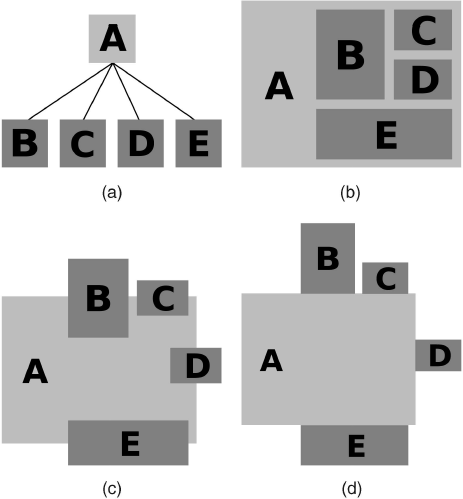
\includegraphics[width=0.8\linewidth]{pictures/5473227-fig-2-source-hires.png}
\caption{(a) explicit node-link layout. (b) implicit node-link by inclusion. (c)  implicit node-link by overlap. (d)  implicit node-link by adjacency. These figures display the same system. Courtesy of Schulz et al. \cite{schulz2011design}} \label{fig:compare}
\end{figure}

\section{Complementary Material}
Although the core of your survey resides in the classification and surveyed material, your paper does not need to end there. In this section, we discuss some additional options to improve your survey paper. We first focus on collective meta-data and some additional figures to improve the comparison of papers, followed by some options derived from the literature.

%\begin{figure}
%\centering
%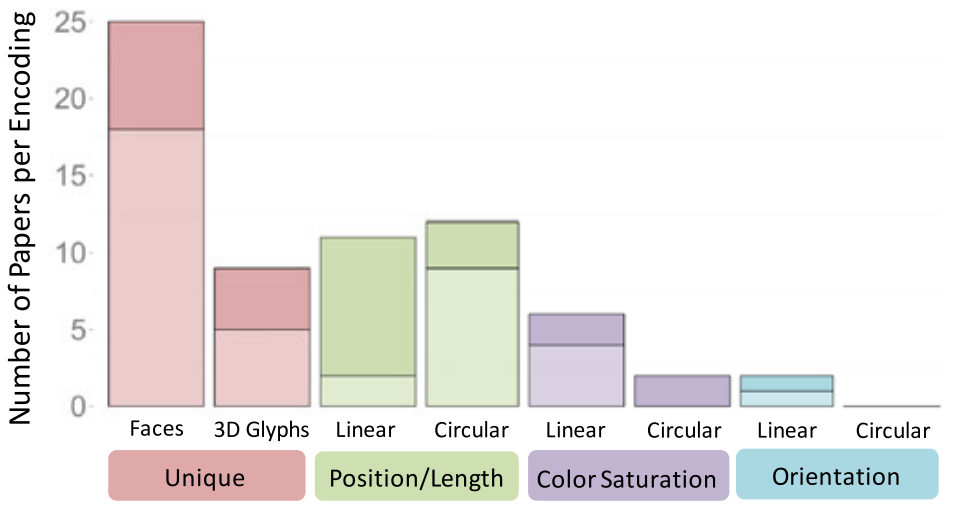
\includegraphics[width=0.8\linewidth]{pictures/glyphEvaluation.png}
%\caption{Ratio of papers evaluating different visual encodings (distinguished by color). Low saturation indicates experiments evaluating design variations of this encoding, and high saturation other experiments (e.g., comparisons to other encodings). Courtesy of Fuchs et al.\ \cite{fuchs2016systematic} } \label{fig:stackedbar}
%\end{figure}

%\begin{figure}
%\centering
%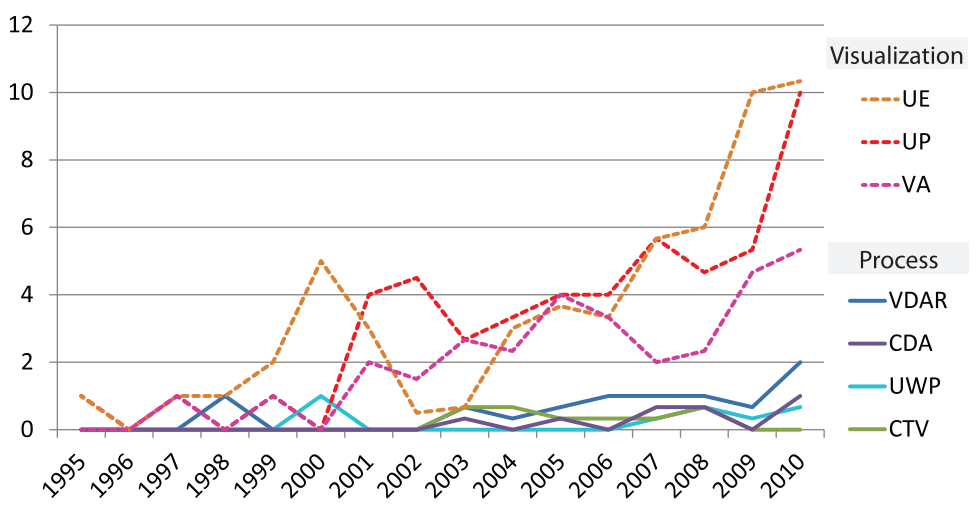
\includegraphics[width=1\linewidth]{pictures/lam2012empirical.png}
%\caption{~} \label{fig:stackedbar}
%\end{figure}



\begin{figure}
\centering
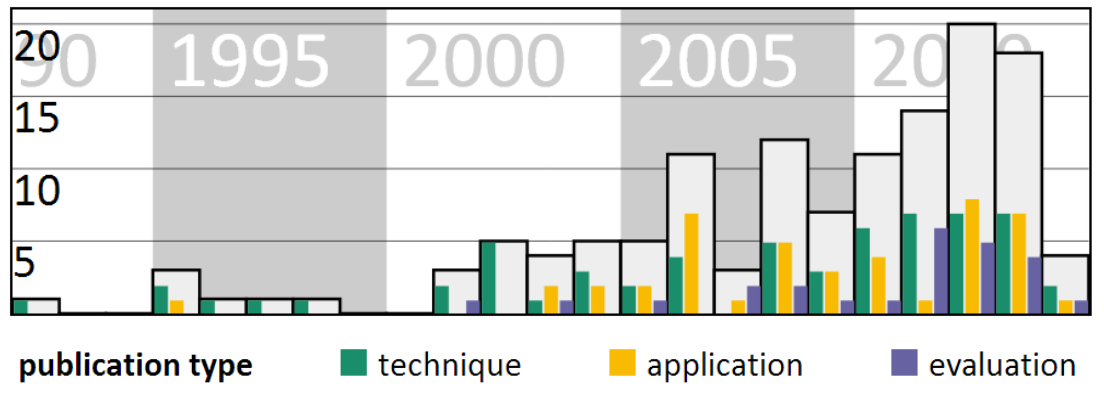
\includegraphics[width=1\linewidth]{pictures/collectiveMetaDataExample.png}
\caption{Yearly number of publications on dynamic graph visualization according to our literature database; light gray bars indicate the total number of publications, colored bars distinguish the publications by type. Courtesy of Beck et al.\ \cite{beck2014state} } \label{fig:bar}
\end{figure}


\begin{table*}[t]
\ra{1.2}
\footnotesize
\centering
\rowcolors{1}{white}{black!3}
\begin{tabularx}{1\textwidth}{|X|X|}
\hline \rowcolor{black!30}
Meta-Data types & Examples \\ \hline
%\rowcolor{black!30}  &  Papers \\ 
Publication year & Beck et al.\ \cite{beck2014state}, Federico et al.\ \cite{federico2016survey} \\
Publication venue & Ko et al.\ \cite{ko2016survey}, Henry et al.\ \cite{henry200720}, Isenberg et al.\ \cite{isenberg2017VPD}\\
Data Origin & Janicke et al.\ \cite{janicke2016visual}, Wanner et al.\ \cite{wanner2014state} \\
Number of citations or impact & Alharbi et al.\ \cite{alharbi2018sos}, Isenberg et al.\ \cite{isenberg2017VPD}, Schneiderman et al.\ \cite{schneiderman2012innovation} \\
Year span of cited literature & McNabb and Laramee \cite{mcnabb2017sos}\\
Evaluation Methods & Isenberg et al.\ \cite{isenberg2013systematic}, Lam et al.\ \cite{lam2012empirical} \\
Literature/Author Relationships & Edmunds et al.\ \cite{edmunds2012surface}, Laramee et al.\ \cite{laramee2004state} \\
Test result comparisons & Lam et al.\ \cite{lam2012empirical}, Zhang et al.\ \cite{zhang2012visual}\\ 
Task Types & Fuchs et al.\ \cite{fuchs2016systematic}, Ahn et al.\ \cite{ahn2014task}, Nusrat and Kerrarcher \cite{nusrat2015task} \\
Additional frameworks & Chen et al.\ \cite{chen2015survey}, Dasgupta et al.\ \cite{dasgupta2012conceptualizing}\\
Interactive Literature Browsers & Beck et al.\ \cite{beck2016visual}, Kucher et al.\ \cite{kucher2015text}\\
\hline
\multicolumn{2}{|m{15.2cm}|}{\centering \textbf{Any un-used classification dimensions (refer to Section \ref{sec:identify})}}\\ \hline
\multicolumn{2}{|m{15.2cm}|}{\small Examples: Visual Design \cite{tong2018storytelling}, Data Set Size , Data Characteristics \cite{janicke2016visual, wanner2014state}, Data Dimensionality  \cite{isenberg2013systematic, fuchs2016systematic} Keywords \cite{isenberg2017visualization}, Pipeline classification \cite{liu2017visualizing}, Feature Comparison \cite{brezovsky2013software}, Supplementary Material Classification \cite{chavent2011gpu, gehlenborg2010visualization, secrier2013visualizing}.}\\


\hline
\end{tabularx}
\caption{A shortlist of potential collective and comparative meta-data.} \label{table:metaTable}
\end{table*}
\subsection{Figures}
As well as presenting some of the work from the summarized papers, figures can be used to enhance understanding of the presented concepts. Bach et al.\ provide an excellent example with hand-drawn illustrations of operations for space-time cube flattening operations (Figure \ref{fig:sto}) \cite{bach2014review}. Hadlak et al.\ present different facets of graph-structured data that are commonly visualized on the survey of multi-faceted graph visualization \cite{hadlak2015survey}. Figures can be used to present more than just an introduction to a concept. Caserta and Zendra, present a comparison of similar systems using different visual techniques to give a comparative view \cite{caserta2011visualization}. Schulz et al.\ present a similar example in their design space of implicit hierarchy visualization \cite{schulz2011design} (Figure \ref{fig:compare}). Borgo et al.\ use comparisons to present visual variables, as well as their glyph design criteria in their glyph-based visualization survey \cite{borgo2013glyph}.  Javed and Elmqvist use figures to present the differences between composite visualization using a scatter plot and bar graph as examples \cite{javed2012exploring}. Vehlow et al.\ present something similar in their state of the art in visualizing group structures in graphs \cite{vehlow2015state}. Tominski et al.'s duology of surveys on interactive lenses in visualization provide good examples of comparative views of techniques and a depiction of an interactive lens technique \cite{tominski2014survey,tominski2016interactive}.

Mentioned in Section \ref{sec:overview}, figures can be used to break down your dimensions. For example if you use a pipeline, presenting it as an image is a useful approach in making sure the reader understands the concept. Chi use this concept to present the information visualization data state reference model, which they use to create a taxonomy of visualization techniques \cite{chi2000taxonomy}. Cottam et al.\ superimpose sources of dynamics onto Chen et al.'s information visualization pipeline \cite{cottam2012watch,card1999readings}. Landesberger et al.\ present their scope and organization in the form of a venn diagram, looking at the main components of visual analysis of large graphs \cite{von2011visual}. Wagner et al.\ present a pipeline depicting the scope and organization of the paper reviewing malware systems \cite{wagner2015survey}. 
For more information on frameworks, Wang et al.\ present a survey on visual analytics pipelines which may be a good starting point \cite{wang2016survey}.

\subsection{Collective Meta-Data for Comparison}
A full survey can occupy more than twice the length of most research papers, and therefore pacing is very important. In order to facilitate comparison of research literature and enhance the sections, you can use the collective meta data to present interesting observations and trends in the literature and make comparisons.

A common set of meta-data to visualize is a \textit{distribution of the literature}. Beck et al.\ present a histogram to present the number of literature papers per year, with the publication type distribution mapped to color \cite{beck2014state}. Federico et al.\ also present a histogram of literature distributed by the year \cite{federico2016survey}. Both of these are very prevalent and are often presented together, for example, Blumenstein et al.\  present a stacked bar chart to display the selected literature's venue, stacked based on the publication year \cite{blumenstein2016evaluating}. 

Another common example comes with the \textit{venues} (conferences or journals for example). Ko et al.\ use a histogram to present this in their survey paper \cite{ko2016survey}.  Lipsa et al.\ present a line chart to present the distribution of papers amongst years and their venues \cite{lipsa2012visualization}.
Rather than looking at the venue, Janicke et al.\ break up the reviewed literature by the \textit{field origin} (visualization or digital humanities) \cite{janicke2016visual}. Alharbi and Laramee compare the number of methods presented in a paper against the \textit{number of citations} using a bar graph. They also present a word cloud of their focus papers to present the differences in the vocabulary used within each \cite{alharbi2018sos}. Isenberg et al.\ produce a line chart depicting \textit{paper counts per year}, showing trends within each publication venue \cite{isenberg2017VPD}. Schneiderman et al.\ provide a similar example, presenting paper counts for three types of tree innovations \cite{schneiderman2012innovation}.
McNabb and Laramee present a gantt chart depicting the \textit{time frame for citations} across their reviewed literature, with number of citations mapped to color \cite{mcnabb2017sos}. 

Edmunds et al.\ classify their papers using \textit{relationship diagrams} to indicate how concepts are built upon each other \cite{edmunds2012surface}. Laramee et al.\ present a similar hierarchy of related literature, with their presented technique's dimensionality mapped to glyphs \cite{laramee2004state}.

Merino et al.\ produce a sankey diagram to present the relationship between data collection and empirical evaluation in their survey software visualization evaluation \cite{merino2018systematic}.
Henry et al.\ present a  wide arrange of meta-data visualization on timelines of paper scope, citation counts, and collaboaration diagrams, as well as more \cite{henry200720}.

A collection of literature can often aid in the creation of a new framework. Even if you do not use this as a dimension in your classification, their is no reason to not include one. Chen et al.\ present a \textit{conceptual pipeline} of traffic data visualization for the survey on the same topic \cite{chen2015survey}. Dasgupta et al.\ end their paper by presenting their visual uncertainty pipeline which they believe extends past the scope of their parallel coordinates survey \cite{dasgupta2012conceptualizing}. Liang and Huang provide multiple models, including a conceptual model of highlighting, and a framework of viewing control \cite{liang2010highlighting}. Lu et al.\  present a predictive visual analytics pipeline for their survey of the same topic \cite{lu2016recent}.  Mattila et al.\ design a pipeline to present the stages of research \cite{mattila2016software}. Zhou et al.\ present a framework depicting an edge-bundling framework for their survey on the same topic \cite{zhou2013edge}.

If you have clearly labeled a scope, you may be able to present some data about options outside of your scope. Fuchs et al.\ use a stacked bar chart to display the ratio of two different \textit{evaluation types}, where a lower saturation indicates experiments evaluating design variations of the marks (those being reviewed) and a higher saturation for other experiments (not reviewed) \cite{fuchs2016systematic}.

 Lam et al.\ review studies presented in their papers  \cite{lam2012empirical}. A bar chart is used to show the distribution between process scenarios and visualization scenarios. They use lines to further evaluate visualization and process scenarios between 1995--2010, by breaking down the scenarios.
Isenberg et al.\ review \textit{evaluation scenarios} using both histograms and a line charts \cite{isenberg2013systematic}.
Zhang et al.\ perform stress tests on the different commercial systems they review, and present them in the form of a bar graph \cite{zhang2012visual}.
 

\subsection{Interactive Literature Browsers}
Interactive literature browsers have become increasingly popular in the realm of visualization survey papers. The browser enables readers to interactively browse the findings of the paper to aid exploration. McNabb and Laramee's SoS paper find 13 literature browsers from the last 5 years, making this a worthwhile consideration.  Although it is possible to produce a unique browser design, we recommend SurVis \cite{beck2016visual} as an option, due to it's open source, and easy-to-implement design.

Kucher and Kerren create their own interactive browser providing the opportunity for users to filter through different text visualization techniques, as well as allowing for user submitted entries \cite{kucher2015text}. Behrisch et al.\ provide a complimentary website to help readers compare matrix plots, as well as present additional meta data on the reviewed literature \cite{matrixreorderingVis}. Dumas et al.\ present a website to review visualization focused on financial data \cite{dumas2014financevis}.

\begin{figure}[t]
\centering
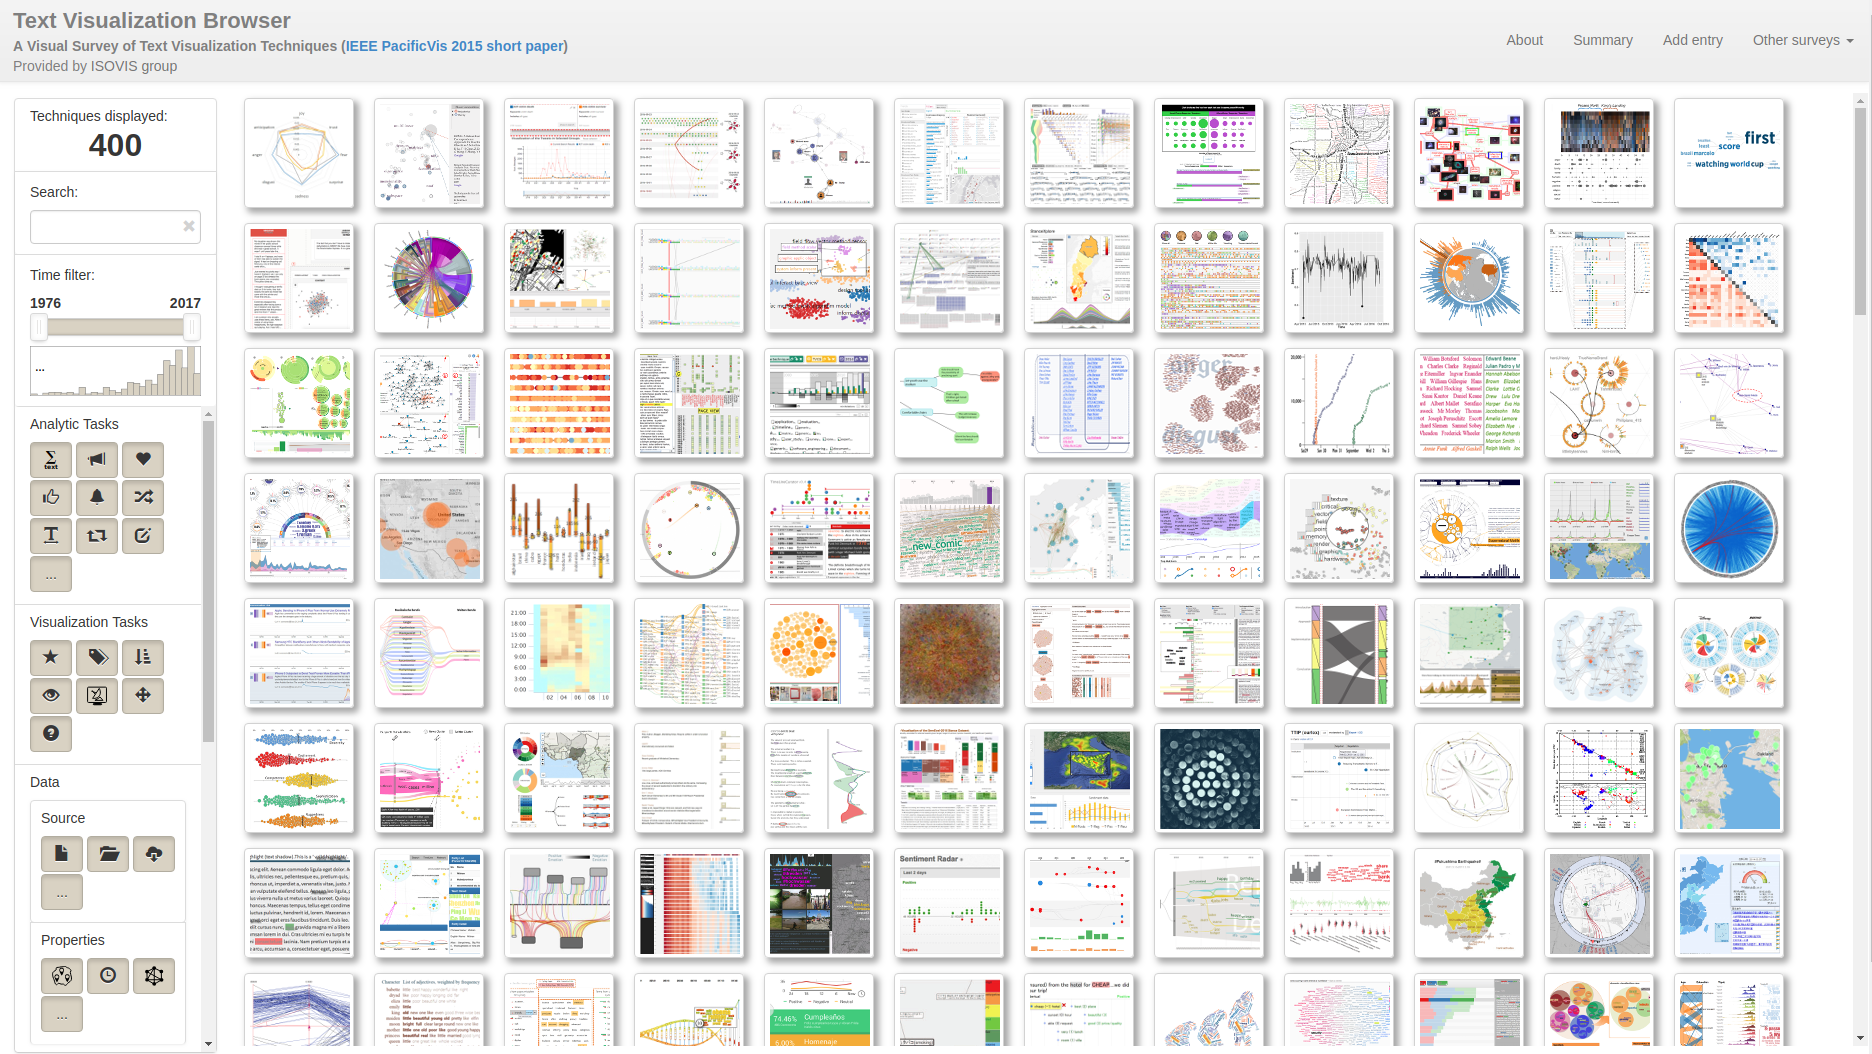
\includegraphics[width=1\linewidth]{pictures/kucherkerren.png}
\caption{Kucher and Kerren's interactive literature browser . 
%\url{http://textvis.lnu.se}
 \cite{kucher2015text}} \label{fig:bar}
\end{figure}

\section{Discussion and Future Challenges} \label{sec:fut}
The discussion and future challenges sections are critical areas within survey papers. The section summarizes any challenges presented in the research papers in generalized terms. By the end of this section, readers could clearly understand what directions should be taken to further the field. If you are having trouble finding the content, domain expert feedback can be used to draw out more areas with less work undertaken.

We recommend referring to the classification that you have designed. It is likely that you have noticed trends throughout the compilation process such as missing or less mature areas within your classification dimensions. Two dimensional classifications are very good at pointing out both mature and immature research directions. Look for holes in your classification table or matrix. Your paper summaries can also be used to identify future research topics. If you notice key topics that seem to be missing or less mature (other potential classification dimensions for example), this is also worth mentioning. Look out for the following when developing your discussion: 1) Empty spaces in the classification table, 2) mature areas with dense research, 3) temporal trends such as early pioneers in the field and trends in only the last few years and 4) trends in publication venues.

\section{Conclusions}
We provide starting point guidelines with a flexible template for the reader to follow in order to produce a full visualization survey paper. The paper offers step-by-step instructions in order to guide the reader through each section of a typical survey, as well as additional considerations that need to be made during the writing cycle. The paper reviews what we consider essential topics and supplementary options that can be used to improve the quality of a survey paper and increase the chance of succeeding through the review process.